% Options for packages loaded elsewhere
\PassOptionsToPackage{unicode}{hyperref}
\PassOptionsToPackage{hyphens}{url}
%
\documentclass[
]{article}
\usepackage{lmodern}
\usepackage{amssymb,amsmath}
\usepackage{ifxetex,ifluatex}
\ifnum 0\ifxetex 1\fi\ifluatex 1\fi=0 % if pdftex
  \usepackage[T1]{fontenc}
  \usepackage[utf8]{inputenc}
  \usepackage{textcomp} % provide euro and other symbols
\else % if luatex or xetex
  \usepackage{unicode-math}
  \defaultfontfeatures{Scale=MatchLowercase}
  \defaultfontfeatures[\rmfamily]{Ligatures=TeX,Scale=1}
\fi
% Use upquote if available, for straight quotes in verbatim environments
\IfFileExists{upquote.sty}{\usepackage{upquote}}{}
\IfFileExists{microtype.sty}{% use microtype if available
  \usepackage[]{microtype}
  \UseMicrotypeSet[protrusion]{basicmath} % disable protrusion for tt fonts
}{}
\makeatletter
\@ifundefined{KOMAClassName}{% if non-KOMA class
  \IfFileExists{parskip.sty}{%
    \usepackage{parskip}
  }{% else
    \setlength{\parindent}{0pt}
    \setlength{\parskip}{6pt plus 2pt minus 1pt}}
}{% if KOMA class
  \KOMAoptions{parskip=half}}
\makeatother
\usepackage{xcolor}
\IfFileExists{xurl.sty}{\usepackage{xurl}}{} % add URL line breaks if available
\IfFileExists{bookmark.sty}{\usepackage{bookmark}}{\usepackage{hyperref}}
\hypersetup{
  pdftitle={Col de la Porte},
  hidelinks,
  pdfcreator={LaTeX via pandoc}}
\urlstyle{same} % disable monospaced font for URLs
\usepackage[margin=1in]{geometry}
\usepackage{longtable,booktabs}
% Correct order of tables after \paragraph or \subparagraph
\usepackage{etoolbox}
\makeatletter
\patchcmd\longtable{\par}{\if@noskipsec\mbox{}\fi\par}{}{}
\makeatother
% Allow footnotes in longtable head/foot
\IfFileExists{footnotehyper.sty}{\usepackage{footnotehyper}}{\usepackage{footnote}}
\makesavenoteenv{longtable}
\usepackage{graphicx}
\makeatletter
\def\maxwidth{\ifdim\Gin@nat@width>\linewidth\linewidth\else\Gin@nat@width\fi}
\def\maxheight{\ifdim\Gin@nat@height>\textheight\textheight\else\Gin@nat@height\fi}
\makeatother
% Scale images if necessary, so that they will not overflow the page
% margins by default, and it is still possible to overwrite the defaults
% using explicit options in \includegraphics[width, height, ...]{}
\setkeys{Gin}{width=\maxwidth,height=\maxheight,keepaspectratio}
% Set default figure placement to htbp
\makeatletter
\def\fps@figure{htbp}
\makeatother
\setlength{\emergencystretch}{3em} % prevent overfull lines
\providecommand{\tightlist}{%
  \setlength{\itemsep}{0pt}\setlength{\parskip}{0pt}}
\setcounter{secnumdepth}{-\maxdimen} % remove section numbering
\newlength{\cslhangindent}
\setlength{\cslhangindent}{1.5em}
\newenvironment{cslreferences}%
  {\setlength{\parindent}{0pt}%
  \everypar{\setlength{\hangindent}{\cslhangindent}}\ignorespaces}%
  {\par}

\title{Col de la Porte}
\author{}
\date{\vspace{-2.5em}}

\begin{document}
\maketitle

\hypertarget{model-geotop-v3.0}{%
\paragraph{Model: GEOtop v3.0}\label{model-geotop-v3.0}}

Compiler: gcc version 4.8.4 (Ubuntu
4.8.4-2ubuntu1\textasciitilde14.04.1) Processor: Intel(R) Core(TM)
i7-5500U CPU @ 2.40GHz Author: Stefano Endrizzi
(\href{mailto:stefano.end@gmail.com}{\nolinkurl{stefano.end@gmail.com}}),Emanuele
Cordano
(\href{mailto:emanuele.cordano@rendena100.eu}{\nolinkurl{emanuele.cordano@rendena100.eu}})
Date: 25-11-2016

\hypertarget{name-coldelaporte}{%
\paragraph{Name: ColdelaPorte}\label{name-coldelaporte}}

Description: Simulation 1D over the Col de la Porte dataset to test the
capability of GEOotp to simulate snow depth, snow water equivalent, soil
temperature.

\hypertarget{results-published-in}{%
\paragraph{Results published in:}\label{results-published-in}}

First result with GEOtop v 2.0 are illustrated in the report XXX
(Endrizzi et al. (2014) , supplemantary material). The following
simulated variables have been tested against observations:

\begin{itemize}
\item
  Liquid Precipitation Intensity (Rain);
\item
  Solid Precipitation Intensity (Snow);
\item
  Snow Height (Snow Dapth);
\item
  Snow Water Equivalent;
\item
  Soil Temperature at 10 cm depth;
\item
  Soil temparature at 20 cm depth;
\item
  Soil Temparature at 50 cm depth;
\item
  Surface Temparature ;
\item
  Albedo .
\end{itemize}

\hypertarget{simulation-duration}{%
\paragraph{Simulation duration:}\label{simulation-duration}}

\begin{verbatim}
InitDateDDMMYYYYhhmm   = 01/01/1997 00:00
EndDateDDMMYYYYhhmm    = 31/12/2011 23:00

### Output:
PointOutputFile = "output-tabs/surface"
\end{verbatim}

\hypertarget{observations}{%
\subsubsection{Observations:}\label{observations}}

Snow heigth mm, Snow Water Equivalent mm(NOT FOUND), T surface C, T soil
10cm C,T soil 20cm C,T soil 50cm C see Morin et al. (2012).

\hypertarget{winter-20012002}{%
\subsubsection{Winter 2001/2002}\label{winter-20012002}}

Here is a comparison plot:

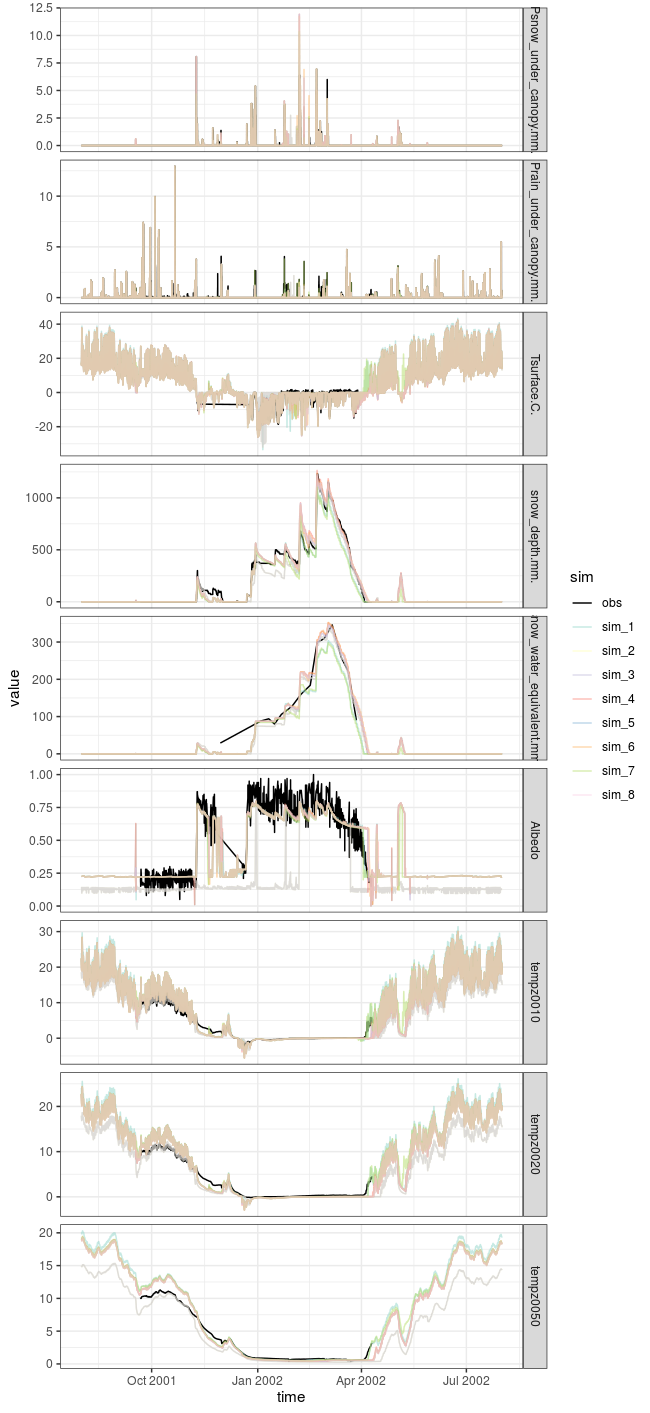
\includegraphics{coldelaporte_v6_files/figure-latex/Winter_2001_2002-1.png}

Goodness of fit:

\begin{longtable}[]{@{}llrrrrrrrrr@{}}
\toprule
sim & gof & Psnow\_under\_canopy.mm. & Prain\_under\_canopy.mm. &
Tsurface.C. & snow\_depth.mm. & snow\_water\_equivalent.mm. & Albedo &
tempz0010 & tempz0020 & tempz0050\tabularnewline
\midrule
\endhead
obs & MAE & 0.02 & 0.03 & 0.00 & 0.00 & 0.00 & 0.00 & 0.00 & 0.00 &
0.00\tabularnewline
obs & RMSE & 0.18 & 0.24 & 0.00 & 0.00 & 0.00 & 0.01 & 0.00 & 0.00 &
0.00\tabularnewline
obs & KGE & 0.84 & 0.89 & 1.00 & 1.00 & 1.00 & 1.00 & 1.00 & 1.00 &
1.00\tabularnewline
sim\_1 & MAE & 0.04 & 0.09 & 1.77 & 45.53 & 20.64 & 0.07 & 0.88 & 0.89 &
0.64\tabularnewline
sim\_1 & RMSE & 0.28 & 0.44 & 2.73 & 67.38 & 27.11 & 0.10 & 1.48 & 1.30
& 1.01\tabularnewline
sim\_1 & KGE & 0.53 & 0.62 & 0.75 & 0.84 & 0.82 & 0.85 & 0.68 & 0.73 &
0.76\tabularnewline
sim\_2 & MAE & 0.05 & 0.11 & 2.55 & 42.79 & 17.41 & 0.27 & 0.59 & 0.72 &
0.71\tabularnewline
sim\_2 & RMSE & 0.27 & 0.50 & 3.84 & 68.66 & 21.39 & 0.37 & 1.05 & 1.08
& 0.93\tabularnewline
sim\_2 & KGE & 0.54 & 0.51 & 0.75 & 0.90 & 0.96 & 0.28 & 0.85 & 0.79 &
0.80\tabularnewline
sim\_3 & MAE & 0.05 & 0.11 & 2.55 & 42.79 & 17.41 & 0.27 & 0.59 & 0.72 &
0.71\tabularnewline
sim\_3 & RMSE & 0.27 & 0.50 & 3.84 & 68.66 & 21.39 & 0.37 & 1.05 & 1.08
& 0.93\tabularnewline
sim\_3 & KGE & 0.54 & 0.51 & 0.75 & 0.90 & 0.96 & 0.28 & 0.85 & 0.79 &
0.80\tabularnewline
sim\_4 & MAE & 0.05 & 0.11 & 1.93 & 35.66 & 16.85 & 0.07 & 0.93 & 0.95 &
0.67\tabularnewline
sim\_4 & RMSE & 0.34 & 0.50 & 2.72 & 58.18 & 24.02 & 0.10 & 1.58 & 1.36
& 0.96\tabularnewline
sim\_4 & KGE & 0.36 & 0.52 & 0.77 & 0.92 & 0.92 & 0.83 & 0.70 & 0.74 &
0.79\tabularnewline
sim\_5 & MAE & 0.05 & 0.11 & 1.96 & 32.75 & 15.86 & 0.07 & 0.92 & 0.94 &
0.66\tabularnewline
sim\_5 & RMSE & 0.34 & 0.50 & 2.88 & 53.19 & 23.34 & 0.11 & 1.56 & 1.34
& 0.94\tabularnewline
sim\_5 & KGE & 0.35 & 0.52 & 0.74 & 0.96 & 0.94 & 0.83 & 0.71 & 0.75 &
0.80\tabularnewline
sim\_6 & MAE & 0.05 & 0.11 & 2.12 & 33.01 & 17.50 & 0.07 & 0.92 & 0.93 &
0.64\tabularnewline
sim\_6 & RMSE & 0.35 & 0.50 & 3.21 & 52.25 & 25.18 & 0.11 & 1.56 & 1.33
& 0.93\tabularnewline
sim\_6 & KGE & 0.30 & 0.52 & 0.69 & 0.95 & 0.91 & 0.82 & 0.71 & 0.75 &
0.80\tabularnewline
sim\_7 & MAE & 0.04 & 0.11 & 1.97 & 53.33 & 25.45 & 0.07 & 0.88 & 0.90 &
0.62\tabularnewline
sim\_7 & RMSE & 0.30 & 0.50 & 2.88 & 78.68 & 30.72 & 0.10 & 1.48 & 1.28
& 0.97\tabularnewline
sim\_7 & KGE & 0.56 & 0.54 & 0.75 & 0.80 & 0.82 & 0.84 & 0.69 & 0.74 &
0.77\tabularnewline
sim\_8 & MAE & 0.05 & 0.11 & 1.96 & 32.75 & 15.86 & 0.07 & 0.92 & 0.94 &
0.66\tabularnewline
sim\_8 & RMSE & 0.34 & 0.50 & 2.88 & 53.19 & 23.34 & 0.11 & 1.56 & 1.34
& 0.94\tabularnewline
sim\_8 & KGE & 0.35 & 0.52 & 0.74 & 0.96 & 0.94 & 0.83 & 0.71 & 0.75 &
0.80\tabularnewline
\bottomrule
\end{longtable}

\hypertarget{winter-20022003}{%
\subsubsection{Winter 2002/2003}\label{winter-20022003}}

Here is a comparison plot:

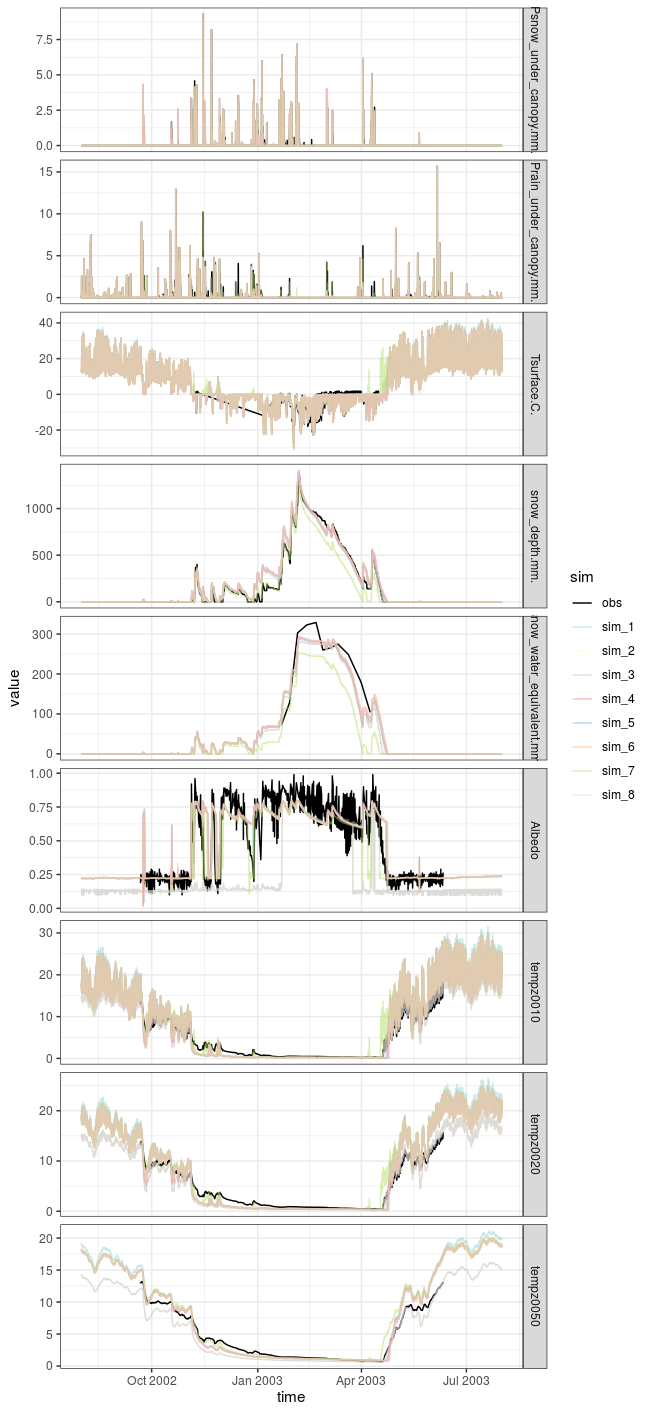
\includegraphics{coldelaporte_v6_files/figure-latex/Winter_2002_2003-1.png}

Goodness of fit:

\begin{longtable}[]{@{}llrrrrrrrrr@{}}
\toprule
sim & gof & Psnow\_under\_canopy.mm. & Prain\_under\_canopy.mm. &
Tsurface.C. & snow\_depth.mm. & snow\_water\_equivalent.mm. & Albedo &
tempz0010 & tempz0020 & tempz0050\tabularnewline
\midrule
\endhead
obs & MAE & 0.03 & 0.05 & 0.00 & 0.00 & 0.00 & 0.00 & 0.00 & 0.00 &
0.00\tabularnewline
obs & RMSE & 0.25 & 0.37 & 0.00 & 0.00 & 0.00 & 0.01 & 0.00 & 0.00 &
0.00\tabularnewline
obs & KGE & 0.75 & 0.81 & 1.00 & 1.00 & 1.00 & 1.00 & 1.00 & 1.00 &
1.00\tabularnewline
sim\_1 & MAE & 0.07 & 0.13 & 1.59 & 41.62 & 33.77 & 0.07 & 1.45 & 1.41 &
0.90\tabularnewline
sim\_1 & RMSE & 0.40 & 0.61 & 2.09 & 70.42 & 40.76 & 0.12 & 2.36 & 2.11
& 1.33\tabularnewline
sim\_1 & KGE & 0.35 & 0.48 & 0.88 & 0.90 & 0.85 & 0.85 & 0.56 & 0.59 &
0.72\tabularnewline
sim\_2 & MAE & 0.07 & 0.14 & 1.82 & 35.17 & 32.94 & 0.23 & 0.85 & 1.02 &
0.92\tabularnewline
sim\_2 & RMSE & 0.34 & 0.66 & 2.57 & 60.59 & 41.72 & 0.32 & 1.23 & 1.36
& 1.18\tabularnewline
sim\_2 & KGE & 0.46 & 0.37 & 0.84 & 0.93 & 0.86 & 0.35 & 0.84 & 0.81 &
0.79\tabularnewline
sim\_3 & MAE & 0.07 & 0.14 & 1.82 & 35.17 & 32.94 & 0.23 & 0.85 & 1.02 &
0.92\tabularnewline
sim\_3 & RMSE & 0.34 & 0.66 & 2.57 & 60.59 & 41.72 & 0.32 & 1.23 & 1.36
& 1.18\tabularnewline
sim\_3 & KGE & 0.46 & 0.37 & 0.84 & 0.93 & 0.86 & 0.35 & 0.84 & 0.81 &
0.79\tabularnewline
sim\_4 & MAE & 0.08 & 0.15 & 1.92 & 42.58 & 31.85 & 0.07 & 1.43 & 1.39 &
0.87\tabularnewline
sim\_4 & RMSE & 0.45 & 0.67 & 2.65 & 73.21 & 38.24 & 0.12 & 2.34 & 2.06
& 1.25\tabularnewline
sim\_4 & KGE & 0.25 & 0.37 & 0.85 & 0.87 & 0.86 & 0.85 & 0.58 & 0.61 &
0.74\tabularnewline
sim\_5 & MAE & 0.08 & 0.15 & 1.87 & 42.80 & 30.10 & 0.07 & 1.39 & 1.35 &
0.84\tabularnewline
sim\_5 & RMSE & 0.45 & 0.67 & 2.59 & 74.92 & 35.98 & 0.12 & 2.27 & 2.00
& 1.20\tabularnewline
sim\_5 & KGE & 0.25 & 0.37 & 0.86 & 0.86 & 0.87 & 0.85 & 0.60 & 0.62 &
0.75\tabularnewline
sim\_6 & MAE & 0.08 & 0.15 & 1.85 & 42.42 & 29.76 & 0.07 & 1.39 & 1.34 &
0.84\tabularnewline
sim\_6 & RMSE & 0.45 & 0.67 & 2.56 & 74.95 & 35.42 & 0.12 & 2.26 & 1.98
& 1.19\tabularnewline
sim\_6 & KGE & 0.25 & 0.37 & 0.87 & 0.86 & 0.87 & 0.85 & 0.60 & 0.62 &
0.75\tabularnewline
sim\_7 & MAE & 0.07 & 0.15 & 1.80 & 52.91 & 71.13 & 0.07 & 1.49 & 1.45 &
1.00\tabularnewline
sim\_7 & RMSE & 0.40 & 0.68 & 2.50 & 89.37 & 82.87 & 0.10 & 2.51 & 2.23
& 1.51\tabularnewline
sim\_7 & KGE & 0.42 & 0.40 & 0.85 & 0.77 & 0.66 & 0.85 & 0.54 & 0.57 &
0.68\tabularnewline
sim\_8 & MAE & 0.08 & 0.15 & 1.87 & 42.80 & 30.10 & 0.07 & 1.39 & 1.35 &
0.84\tabularnewline
sim\_8 & RMSE & 0.45 & 0.67 & 2.59 & 74.92 & 35.98 & 0.12 & 2.27 & 2.00
& 1.20\tabularnewline
sim\_8 & KGE & 0.25 & 0.37 & 0.86 & 0.86 & 0.87 & 0.85 & 0.60 & 0.62 &
0.75\tabularnewline
\bottomrule
\end{longtable}

\hypertarget{winter-20032004}{%
\subsubsection{Winter 2003/2004}\label{winter-20032004}}

Here is a comparison plot:

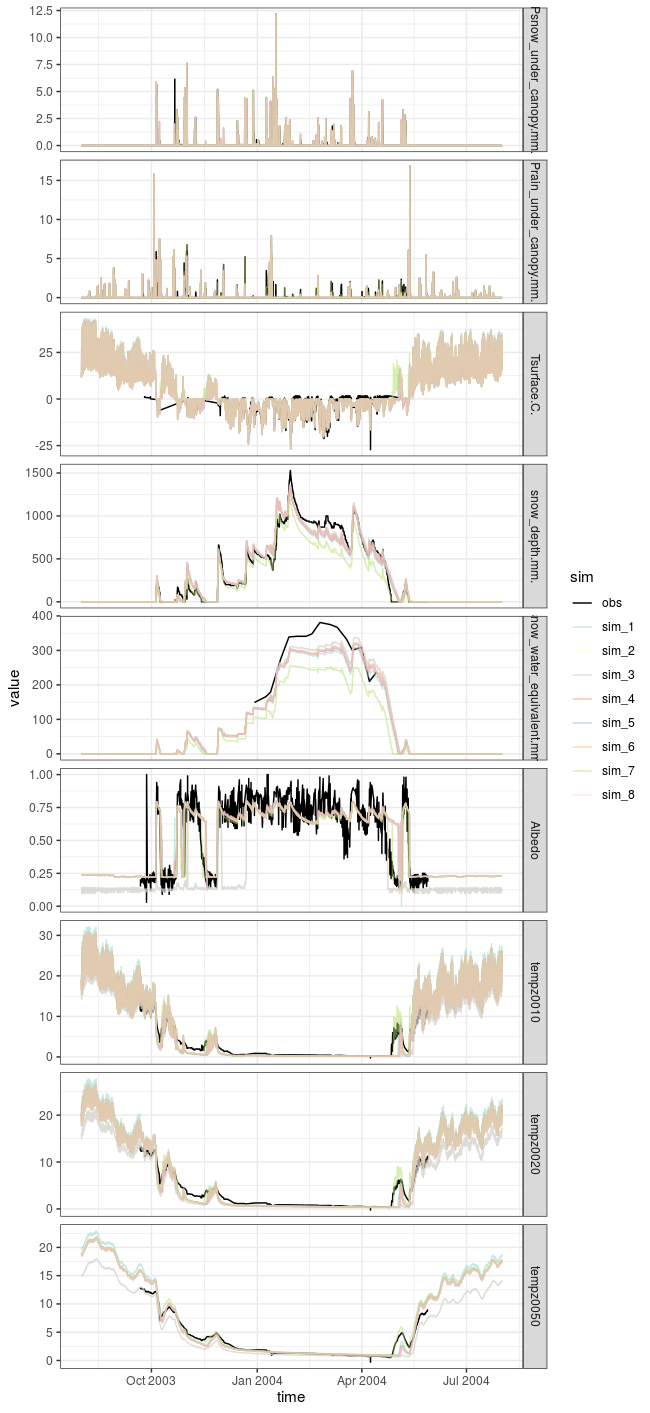
\includegraphics{coldelaporte_v6_files/figure-latex/Winter_2003_2004-1.png}

Goodness of fit:

\begin{longtable}[]{@{}llrrrrrrrrr@{}}
\toprule
sim & gof & Psnow\_under\_canopy.mm. & Prain\_under\_canopy.mm. &
Tsurface.C. & snow\_depth.mm. & snow\_water\_equivalent.mm. & Albedo &
tempz0010 & tempz0020 & tempz0050\tabularnewline
\midrule
\endhead
obs & MAE & 0.04 & 0.04 & 0.00 & 0.00 & 0.00 & 0.00 & 0.00 & 0.00 &
0.00\tabularnewline
obs & RMSE & 0.28 & 0.35 & 0.00 & 0.00 & 0.00 & 0.01 & 0.00 & 0.00 &
0.00\tabularnewline
obs & KGE & 0.75 & 0.74 & 1.00 & 1.00 & 1.00 & 1.00 & 1.00 & 1.00 &
1.00\tabularnewline
sim\_1 & MAE & 0.08 & 0.10 & 1.43 & 66.56 & 46.90 & 0.09 & 0.94 & 0.95 &
0.60\tabularnewline
sim\_1 & RMSE & 0.43 & 0.55 & 1.99 & 91.80 & 52.41 & 0.14 & 1.66 & 1.49
& 0.99\tabularnewline
sim\_1 & KGE & 0.38 & 0.39 & 0.90 & 0.90 & 0.69 & 0.77 & 0.73 & 0.74 &
0.82\tabularnewline
sim\_2 & MAE & 0.08 & 0.11 & 1.61 & 57.29 & 34.45 & 0.18 & 0.96 & 1.09 &
0.93\tabularnewline
sim\_2 & RMSE & 0.41 & 0.57 & 2.33 & 83.30 & 39.74 & 0.27 & 1.60 & 1.56
& 1.27\tabularnewline
sim\_2 & KGE & 0.44 & 0.33 & 0.88 & 0.94 & 0.78 & 0.53 & 0.66 & 0.66 &
0.73\tabularnewline
sim\_3 & MAE & 0.08 & 0.11 & 1.61 & 57.29 & 34.45 & 0.18 & 0.96 & 1.09 &
0.93\tabularnewline
sim\_3 & RMSE & 0.41 & 0.57 & 2.33 & 83.30 & 39.74 & 0.27 & 1.60 & 1.56
& 1.27\tabularnewline
sim\_3 & KGE & 0.44 & 0.33 & 0.88 & 0.94 & 0.78 & 0.53 & 0.66 & 0.66 &
0.73\tabularnewline
sim\_4 & MAE & 0.09 & 0.11 & 1.68 & 64.22 & 41.68 & 0.09 & 0.96 & 0.97 &
0.58\tabularnewline
sim\_4 & RMSE & 0.48 & 0.58 & 2.41 & 88.85 & 47.61 & 0.14 & 1.69 & 1.49
& 0.93\tabularnewline
sim\_4 & KGE & 0.31 & 0.33 & 0.87 & 0.92 & 0.71 & 0.76 & 0.74 & 0.75 &
0.85\tabularnewline
sim\_5 & MAE & 0.09 & 0.11 & 1.66 & 62.61 & 40.29 & 0.09 & 0.96 & 0.97 &
0.58\tabularnewline
sim\_5 & RMSE & 0.48 & 0.58 & 2.38 & 86.67 & 46.15 & 0.14 & 1.69 & 1.49
& 0.93\tabularnewline
sim\_5 & KGE & 0.31 & 0.33 & 0.87 & 0.92 & 0.72 & 0.76 & 0.74 & 0.75 &
0.86\tabularnewline
sim\_6 & MAE & 0.09 & 0.11 & 1.66 & 61.65 & 39.60 & 0.09 & 0.97 & 0.98 &
0.59\tabularnewline
sim\_6 & RMSE & 0.48 & 0.58 & 2.37 & 85.53 & 45.38 & 0.14 & 1.70 & 1.50
& 0.94\tabularnewline
sim\_6 & KGE & 0.31 & 0.33 & 0.87 & 0.93 & 0.72 & 0.76 & 0.74 & 0.75 &
0.86\tabularnewline
sim\_7 & MAE & 0.08 & 0.12 & 1.64 & 104.51 & 88.34 & 0.08 & 0.85 & 0.86
& 0.50\tabularnewline
sim\_7 & RMSE & 0.45 & 0.58 & 2.34 & 147.32 & 93.54 & 0.11 & 1.50 & 1.33
& 0.83\tabularnewline
sim\_7 & KGE & 0.42 & 0.37 & 0.88 & 0.71 & 0.55 & 0.84 & 0.72 & 0.75 &
0.81\tabularnewline
sim\_8 & MAE & 0.09 & 0.11 & 1.66 & 62.61 & 40.29 & 0.09 & 0.96 & 0.97 &
0.58\tabularnewline
sim\_8 & RMSE & 0.48 & 0.58 & 2.38 & 86.67 & 46.15 & 0.14 & 1.69 & 1.49
& 0.93\tabularnewline
sim\_8 & KGE & 0.31 & 0.33 & 0.87 & 0.92 & 0.72 & 0.76 & 0.74 & 0.75 &
0.86\tabularnewline
\bottomrule
\end{longtable}

\hypertarget{winter-20042005}{%
\subsubsection{Winter 2004/2005}\label{winter-20042005}}

Here is a comparison plot:

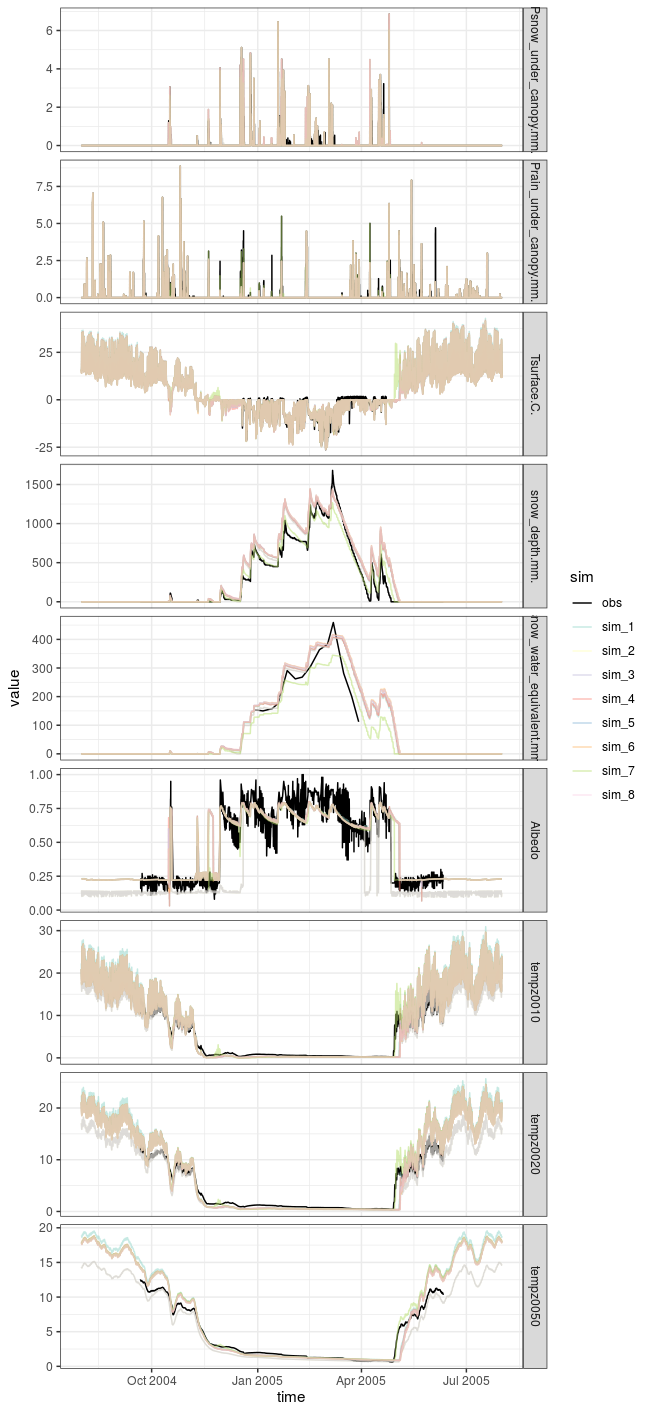
\includegraphics{coldelaporte_v6_files/figure-latex/Winter_2004_2005-1.png}

Goodness of fit:

\begin{longtable}[]{@{}llrrrrrrrrr@{}}
\toprule
sim & gof & Psnow\_under\_canopy.mm. & Prain\_under\_canopy.mm. &
Tsurface.C. & snow\_depth.mm. & snow\_water\_equivalent.mm. & Albedo &
tempz0010 & tempz0020 & tempz0050\tabularnewline
\midrule
\endhead
obs & MAE & 0.03 & 0.04 & 0.00 & 0.00 & 0.00 & 0.00 & 0.00 & 0.00 &
0.00\tabularnewline
obs & RMSE & 0.21 & 0.27 & 0.00 & 0.00 & 0.00 & 0.01 & 0.00 & 0.00 &
0.00\tabularnewline
obs & KGE & 0.80 & 0.88 & 1.00 & 1.00 & 1.00 & 1.00 & 1.00 & 1.00 &
1.00\tabularnewline
sim\_1 & MAE & 0.06 & 0.10 & 1.36 & 89.82 & 43.49 & 0.07 & 1.24 & 1.11 &
0.79\tabularnewline
sim\_1 & RMSE & 0.32 & 0.46 & 1.90 & 140.73 & 58.60 & 0.13 & 2.23 & 1.81
& 1.27\tabularnewline
sim\_1 & KGE & 0.50 & 0.61 & 0.93 & 0.75 & 0.78 & 0.83 & 0.63 & 0.68 &
0.73\tabularnewline
sim\_2 & MAE & 0.06 & 0.11 & 1.70 & 84.29 & 39.49 & 0.12 & 0.71 & 0.80 &
0.78\tabularnewline
sim\_2 & RMSE & 0.32 & 0.50 & 2.45 & 135.89 & 58.18 & 0.18 & 1.35 & 1.29
& 1.07\tabularnewline
sim\_2 & KGE & 0.52 & 0.53 & 0.90 & 0.77 & 0.80 & 0.72 & 0.83 & 0.80 &
0.81\tabularnewline
sim\_3 & MAE & 0.06 & 0.11 & 1.70 & 84.29 & 39.49 & 0.12 & 0.71 & 0.80 &
0.78\tabularnewline
sim\_3 & RMSE & 0.32 & 0.50 & 2.45 & 135.89 & 58.18 & 0.18 & 1.35 & 1.29
& 1.07\tabularnewline
sim\_3 & KGE & 0.52 & 0.53 & 0.90 & 0.77 & 0.80 & 0.72 & 0.83 & 0.80 &
0.81\tabularnewline
sim\_4 & MAE & 0.07 & 0.11 & 1.72 & 93.94 & 43.76 & 0.07 & 1.22 & 1.09 &
0.75\tabularnewline
sim\_4 & RMSE & 0.35 & 0.51 & 2.47 & 146.20 & 58.95 & 0.13 & 2.22 & 1.77
& 1.18\tabularnewline
sim\_4 & KGE & 0.44 & 0.53 & 0.90 & 0.73 & 0.78 & 0.83 & 0.65 & 0.70 &
0.77\tabularnewline
sim\_5 & MAE & 0.07 & 0.11 & 1.69 & 99.36 & 47.94 & 0.07 & 1.21 & 1.08 &
0.74\tabularnewline
sim\_5 & RMSE & 0.35 & 0.51 & 2.41 & 154.36 & 63.80 & 0.13 & 2.18 & 1.75
& 1.16\tabularnewline
sim\_5 & KGE & 0.44 & 0.53 & 0.90 & 0.71 & 0.76 & 0.83 & 0.66 & 0.71 &
0.78\tabularnewline
sim\_6 & MAE & 0.07 & 0.11 & 1.68 & 99.98 & 48.91 & 0.07 & 1.21 & 1.08 &
0.74\tabularnewline
sim\_6 & RMSE & 0.35 & 0.51 & 2.38 & 155.88 & 65.27 & 0.13 & 2.18 & 1.75
& 1.16\tabularnewline
sim\_6 & KGE & 0.44 & 0.53 & 0.91 & 0.71 & 0.76 & 0.83 & 0.66 & 0.72 &
0.78\tabularnewline
sim\_7 & MAE & 0.06 & 0.11 & 1.69 & 44.04 & 39.06 & 0.06 & 1.18 & 1.05 &
0.73\tabularnewline
sim\_7 & RMSE & 0.32 & 0.51 & 2.41 & 79.29 & 48.12 & 0.09 & 2.04 & 1.62
& 1.14\tabularnewline
sim\_7 & KGE & 0.56 & 0.58 & 0.90 & 0.92 & 0.74 & 0.88 & 0.60 & 0.67 &
0.73\tabularnewline
sim\_8 & MAE & 0.07 & 0.11 & 1.69 & 99.36 & 47.94 & 0.07 & 1.21 & 1.08 &
0.74\tabularnewline
sim\_8 & RMSE & 0.35 & 0.51 & 2.41 & 154.36 & 63.80 & 0.13 & 2.18 & 1.75
& 1.16\tabularnewline
sim\_8 & KGE & 0.44 & 0.53 & 0.90 & 0.71 & 0.76 & 0.83 & 0.66 & 0.71 &
0.78\tabularnewline
\bottomrule
\end{longtable}

\hypertarget{winter-20052006}{%
\subsubsection{Winter 2005/2006}\label{winter-20052006}}

Here is a comparison plot:

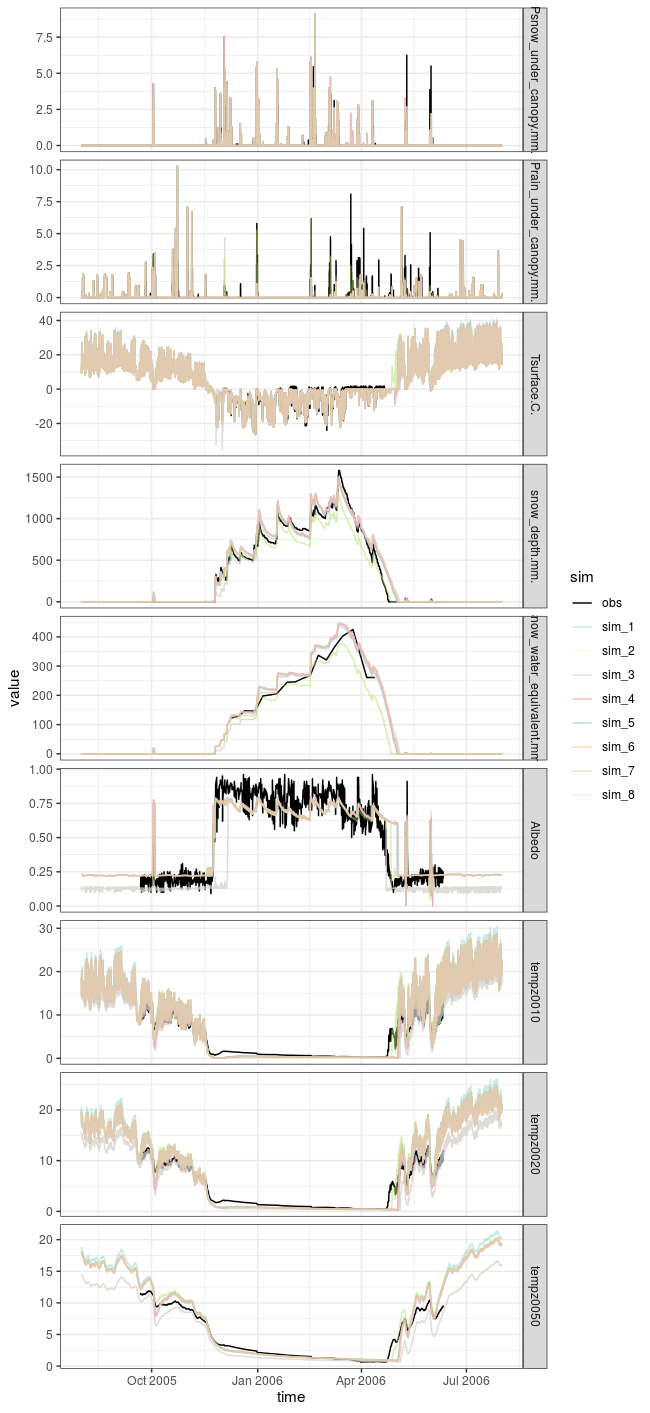
\includegraphics{coldelaporte_v6_files/figure-latex/Winter_2005_2006-1.png}

Goodness of fit:

\begin{longtable}[]{@{}llrrrrrrrrr@{}}
\toprule
sim & gof & Psnow\_under\_canopy.mm. & Prain\_under\_canopy.mm. &
Tsurface.C. & snow\_depth.mm. & snow\_water\_equivalent.mm. & Albedo &
tempz0010 & tempz0020 & tempz0050\tabularnewline
\midrule
\endhead
obs & MAE & 0.03 & 0.04 & 0.00 & 0.00 & 0.00 & 0.00 & 0.00 & 0.00 &
0.00\tabularnewline
obs & RMSE & 0.25 & 0.28 & 0.00 & 0.00 & 0.00 & 0.01 & 0.00 & 0.00 &
0.00\tabularnewline
obs & KGE & 0.72 & 0.81 & 1.00 & 1.00 & 1.00 & 1.00 & 1.00 & 1.00 &
1.00\tabularnewline
sim\_1 & MAE & 0.06 & 0.08 & 1.46 & 49.16 & 18.35 & 0.08 & 1.35 & 1.14 &
0.70\tabularnewline
sim\_1 & RMSE & 0.36 & 0.42 & 1.98 & 75.26 & 22.10 & 0.13 & 2.23 & 1.74
& 1.05\tabularnewline
sim\_1 & KGE & 0.40 & 0.44 & 0.94 & 0.95 & 0.92 & 0.81 & 0.58 & 0.68 &
0.80\tabularnewline
sim\_2 & MAE & 0.07 & 0.09 & 1.89 & 53.49 & 25.23 & 0.10 & 0.93 & 1.07 &
1.07\tabularnewline
sim\_2 & RMSE & 0.38 & 0.46 & 2.80 & 86.55 & 28.77 & 0.14 & 1.60 & 1.61
& 1.46\tabularnewline
sim\_2 & KGE & 0.39 & 0.34 & 0.89 & 0.96 & 0.79 & 0.82 & 0.77 & 0.74 &
0.75\tabularnewline
sim\_3 & MAE & 0.07 & 0.09 & 1.89 & 53.49 & 25.23 & 0.10 & 0.93 & 1.07 &
1.07\tabularnewline
sim\_3 & RMSE & 0.38 & 0.46 & 2.80 & 86.55 & 28.77 & 0.14 & 1.60 & 1.61
& 1.46\tabularnewline
sim\_3 & KGE & 0.39 & 0.34 & 0.89 & 0.96 & 0.79 & 0.82 & 0.77 & 0.74 &
0.75\tabularnewline
sim\_4 & MAE & 0.07 & 0.09 & 1.82 & 52.09 & 22.08 & 0.08 & 1.33 & 1.12 &
0.68\tabularnewline
sim\_4 & RMSE & 0.40 & 0.46 & 2.59 & 80.26 & 26.13 & 0.13 & 2.20 & 1.70
& 1.00\tabularnewline
sim\_4 & KGE & 0.30 & 0.35 & 0.90 & 0.93 & 0.89 & 0.81 & 0.60 & 0.70 &
0.83\tabularnewline
sim\_5 & MAE & 0.07 & 0.09 & 1.78 & 53.81 & 23.61 & 0.08 & 1.30 & 1.10 &
0.67\tabularnewline
sim\_5 & RMSE & 0.40 & 0.46 & 2.53 & 83.45 & 28.00 & 0.13 & 2.15 & 1.67
& 0.98\tabularnewline
sim\_5 & KGE & 0.30 & 0.35 & 0.90 & 0.92 & 0.88 & 0.80 & 0.62 & 0.71 &
0.84\tabularnewline
sim\_6 & MAE & 0.07 & 0.09 & 1.77 & 54.55 & 24.31 & 0.08 & 1.30 & 1.09 &
0.67\tabularnewline
sim\_6 & RMSE & 0.40 & 0.46 & 2.51 & 85.02 & 29.08 & 0.13 & 2.16 & 1.67
& 0.99\tabularnewline
sim\_6 & KGE & 0.30 & 0.35 & 0.90 & 0.92 & 0.87 & 0.80 & 0.62 & 0.71 &
0.84\tabularnewline
sim\_7 & MAE & 0.06 & 0.09 & 1.76 & 62.02 & 26.43 & 0.07 & 1.27 & 1.08 &
0.74\tabularnewline
sim\_7 & RMSE & 0.36 & 0.47 & 2.50 & 100.93 & 36.20 & 0.10 & 2.15 & 1.66
& 1.05\tabularnewline
sim\_7 & KGE & 0.47 & 0.44 & 0.91 & 0.82 & 0.83 & 0.83 & 0.57 & 0.66 &
0.77\tabularnewline
sim\_8 & MAE & 0.07 & 0.09 & 1.78 & 53.81 & 23.61 & 0.08 & 1.30 & 1.10 &
0.67\tabularnewline
sim\_8 & RMSE & 0.40 & 0.46 & 2.53 & 83.45 & 28.00 & 0.13 & 2.15 & 1.67
& 0.98\tabularnewline
sim\_8 & KGE & 0.30 & 0.35 & 0.90 & 0.92 & 0.88 & 0.80 & 0.62 & 0.71 &
0.84\tabularnewline
\bottomrule
\end{longtable}

\hypertarget{winter-20062007}{%
\subsubsection{Winter 2006/2007}\label{winter-20062007}}

Here is a comparison plot:

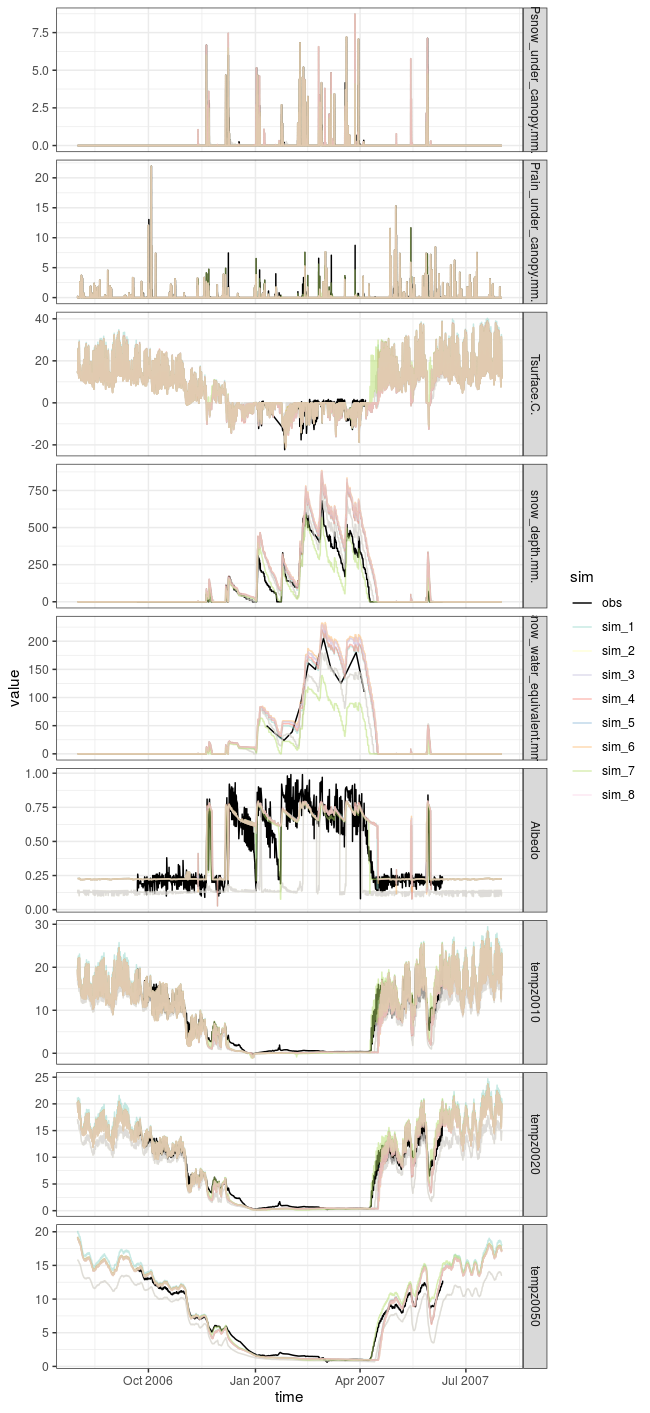
\includegraphics{coldelaporte_v6_files/figure-latex/Winter_2006_2007-1.png}

Goodness of fit:

\begin{longtable}[]{@{}llrrrrrrrrr@{}}
\toprule
sim & gof & Psnow\_under\_canopy.mm. & Prain\_under\_canopy.mm. &
Tsurface.C. & snow\_depth.mm. & snow\_water\_equivalent.mm. & Albedo &
tempz0010 & tempz0020 & tempz0050\tabularnewline
\midrule
\endhead
obs & MAE & 0.03 & 0.06 & 0.00 & 0.00 & 0.00 & 0.00 & 0.00 & 0.00 &
0.00\tabularnewline
obs & RMSE & 0.25 & 0.44 & 0.00 & 0.00 & 0.00 & 0.01 & 0.00 & 0.00 &
0.00\tabularnewline
obs & KGE & 0.70 & 0.80 & 1.00 & 1.00 & 1.00 & 1.00 & 1.00 & 1.00 &
1.00\tabularnewline
sim\_1 & MAE & 0.07 & 0.18 & 1.55 & 58.21 & 20.37 & 0.07 & 0.96 & 0.84 &
0.65\tabularnewline
sim\_1 & RMSE & 0.43 & 0.79 & 2.06 & 101.75 & 25.29 & 0.12 & 1.73 & 1.42
& 0.93\tabularnewline
sim\_1 & KGE & 0.13 & 0.36 & 0.83 & 0.38 & 0.82 & 0.86 & 0.86 & 0.87 &
0.88\tabularnewline
sim\_2 & MAE & 0.07 & 0.20 & 1.87 & 36.46 & 17.21 & 0.19 & 1.52 & 1.35 &
1.33\tabularnewline
sim\_2 & RMSE & 0.37 & 0.82 & 2.72 & 63.92 & 22.07 & 0.28 & 2.25 & 1.91
& 1.68\tabularnewline
sim\_2 & KGE & 0.27 & 0.29 & 0.70 & 0.70 & 0.80 & 0.40 & 0.69 & 0.72 &
0.74\tabularnewline
sim\_3 & MAE & 0.07 & 0.20 & 1.87 & 36.46 & 17.21 & 0.19 & 1.52 & 1.35 &
1.33\tabularnewline
sim\_3 & RMSE & 0.37 & 0.82 & 2.72 & 63.92 & 22.07 & 0.28 & 2.25 & 1.91
& 1.68\tabularnewline
sim\_3 & KGE & 0.27 & 0.29 & 0.70 & 0.70 & 0.80 & 0.40 & 0.69 & 0.72 &
0.74\tabularnewline
sim\_4 & MAE & 0.08 & 0.20 & 1.81 & 60.75 & 22.31 & 0.07 & 1.00 & 0.83 &
0.62\tabularnewline
sim\_4 & RMSE & 0.46 & 0.83 & 2.50 & 104.46 & 27.03 & 0.12 & 1.79 & 1.44
& 0.92\tabularnewline
sim\_4 & KGE & 0.06 & 0.29 & 0.78 & 0.35 & 0.80 & 0.85 & 0.87 & 0.88 &
0.89\tabularnewline
sim\_5 & MAE & 0.08 & 0.20 & 1.77 & 65.18 & 28.96 & 0.07 & 0.98 & 0.83 &
0.61\tabularnewline
sim\_5 & RMSE & 0.46 & 0.83 & 2.47 & 112.13 & 33.77 & 0.12 & 1.80 & 1.46
& 0.92\tabularnewline
sim\_5 & KGE & 0.06 & 0.29 & 0.79 & 0.29 & 0.73 & 0.86 & 0.87 & 0.88 &
0.89\tabularnewline
sim\_6 & MAE & 0.08 & 0.20 & 1.75 & 67.36 & 32.95 & 0.07 & 0.98 & 0.82 &
0.61\tabularnewline
sim\_6 & RMSE & 0.46 & 0.83 & 2.45 & 115.51 & 37.23 & 0.12 & 1.81 & 1.47
& 0.93\tabularnewline
sim\_6 & KGE & 0.06 & 0.29 & 0.79 & 0.27 & 0.69 & 0.86 & 0.87 & 0.88 &
0.90\tabularnewline
sim\_7 & MAE & 0.06 & 0.21 & 1.73 & 29.93 & 44.92 & 0.05 & 0.84 & 0.77 &
0.65\tabularnewline
sim\_7 & RMSE & 0.38 & 0.85 & 2.43 & 53.83 & 52.79 & 0.07 & 1.23 & 1.12
& 0.89\tabularnewline
sim\_7 & KGE & 0.37 & 0.32 & 0.78 & 0.76 & 0.44 & 0.93 & 0.86 & 0.85 &
0.84\tabularnewline
sim\_8 & MAE & 0.08 & 0.20 & 1.77 & 65.18 & 28.96 & 0.07 & 0.98 & 0.83 &
0.61\tabularnewline
sim\_8 & RMSE & 0.46 & 0.83 & 2.47 & 112.13 & 33.77 & 0.12 & 1.80 & 1.46
& 0.92\tabularnewline
sim\_8 & KGE & 0.06 & 0.29 & 0.79 & 0.29 & 0.73 & 0.86 & 0.87 & 0.88 &
0.89\tabularnewline
\bottomrule
\end{longtable}

\hypertarget{winter-20072008}{%
\subsubsection{Winter 2007/2008}\label{winter-20072008}}

Here is a comparison plot:

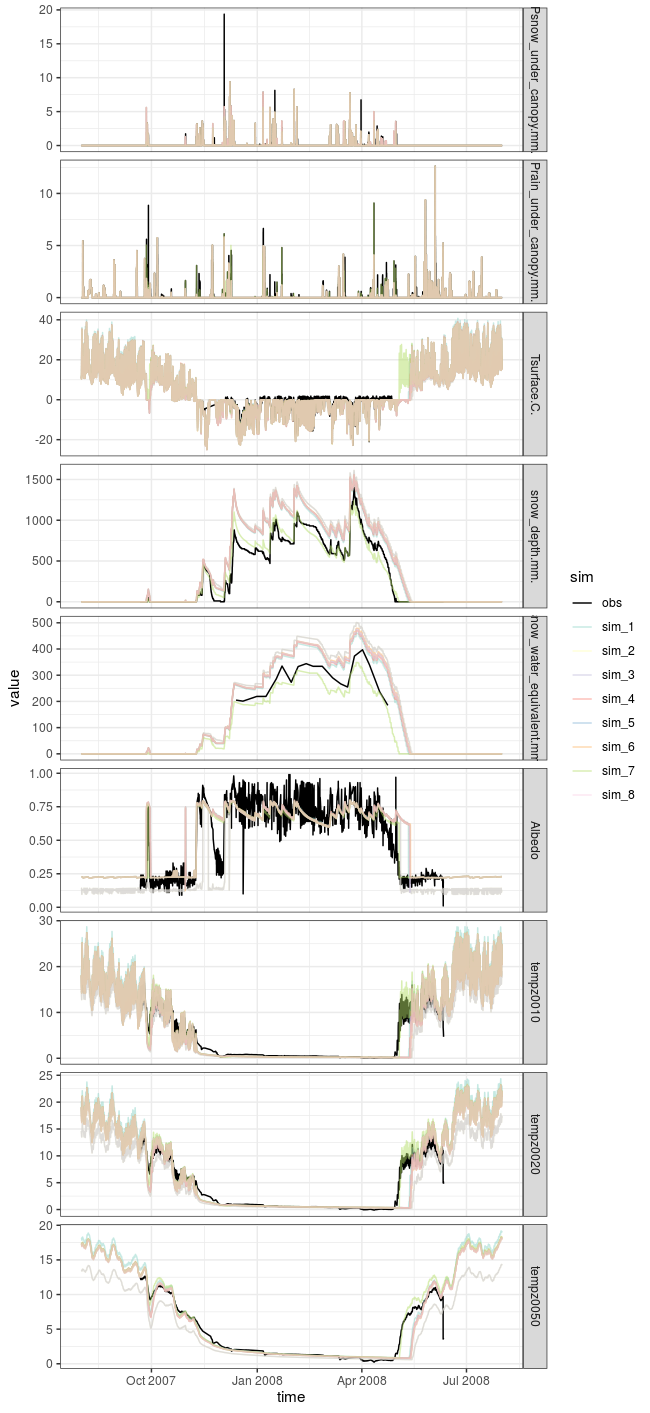
\includegraphics{coldelaporte_v6_files/figure-latex/Winter_2007_2009-1.png}

Goodness of fit:

\begin{longtable}[]{@{}llrrrrrrrrr@{}}
\toprule
sim & gof & Psnow\_under\_canopy.mm. & Prain\_under\_canopy.mm. &
Tsurface.C. & snow\_depth.mm. & snow\_water\_equivalent.mm. & Albedo &
tempz0010 & tempz0020 & tempz0050\tabularnewline
\midrule
\endhead
obs & MAE & 0.04 & 0.04 & 0.00 & 0.00 & 0.00 & 0.00 & 0.00 & 0.00 &
0.00\tabularnewline
obs & RMSE & 0.32 & 0.29 & 0.00 & 0.00 & 0.00 & 0.01 & 0.00 & 0.00 &
0.00\tabularnewline
obs & KGE & 0.77 & 0.83 & 1.00 & 1.00 & 1.00 & 1.00 & 1.00 & 1.00 &
1.00\tabularnewline
sim\_1 & MAE & 0.09 & 0.10 & 1.68 & 173.70 & 68.12 & 0.09 & 0.99 & 0.83
& 0.60\tabularnewline
sim\_1 & RMSE & 0.44 & 0.47 & 2.35 & 228.65 & 72.73 & 0.14 & 2.18 & 1.82
& 1.24\tabularnewline
sim\_1 & KGE & 0.48 & 0.49 & 0.69 & 0.50 & 0.74 & 0.80 & 0.82 & 0.88 &
0.92\tabularnewline
sim\_2 & MAE & 0.09 & 0.11 & 1.98 & 218.79 & 98.22 & 0.10 & 1.42 & 1.29
& 1.36\tabularnewline
sim\_2 & RMSE & 0.47 & 0.50 & 2.78 & 278.55 & 103.00 & 0.15 & 2.69 &
2.36 & 2.03\tabularnewline
sim\_2 & KGE & 0.46 & 0.40 & 0.68 & 0.37 & 0.63 & 0.80 & 0.54 & 0.58 &
0.59\tabularnewline
sim\_3 & MAE & 0.09 & 0.11 & 1.98 & 218.79 & 98.22 & 0.10 & 1.42 & 1.29
& 1.36\tabularnewline
sim\_3 & RMSE & 0.47 & 0.50 & 2.78 & 278.55 & 103.00 & 0.15 & 2.69 &
2.36 & 2.03\tabularnewline
sim\_3 & KGE & 0.46 & 0.40 & 0.68 & 0.37 & 0.63 & 0.80 & 0.54 & 0.58 &
0.59\tabularnewline
sim\_4 & MAE & 0.10 & 0.11 & 2.00 & 186.14 & 75.06 & 0.09 & 1.04 & 0.86
& 0.64\tabularnewline
sim\_4 & RMSE & 0.49 & 0.51 & 2.81 & 242.24 & 79.62 & 0.15 & 2.27 & 1.89
& 1.31\tabularnewline
sim\_4 & KGE & 0.41 & 0.41 & 0.67 & 0.47 & 0.72 & 0.79 & 0.81 & 0.86 &
0.90\tabularnewline
sim\_5 & MAE & 0.10 & 0.11 & 1.94 & 190.65 & 79.20 & 0.09 & 1.04 & 0.87
& 0.65\tabularnewline
sim\_5 & RMSE & 0.49 & 0.51 & 2.74 & 247.18 & 83.94 & 0.15 & 2.29 & 1.92
& 1.34\tabularnewline
sim\_5 & KGE & 0.41 & 0.41 & 0.68 & 0.45 & 0.70 & 0.78 & 0.80 & 0.86 &
0.89\tabularnewline
sim\_6 & MAE & 0.10 & 0.11 & 1.93 & 193.21 & 81.43 & 0.09 & 1.05 & 0.87
& 0.65\tabularnewline
sim\_6 & RMSE & 0.49 & 0.51 & 2.73 & 249.93 & 86.21 & 0.15 & 2.30 & 1.93
& 1.35\tabularnewline
sim\_6 & KGE & 0.41 & 0.41 & 0.68 & 0.45 & 0.70 & 0.78 & 0.80 & 0.86 &
0.89\tabularnewline
sim\_7 & MAE & 0.08 & 0.12 & 1.91 & 56.26 & 32.08 & 0.07 & 0.74 & 0.65 &
0.47\tabularnewline
sim\_7 & RMSE & 0.45 & 0.53 & 2.71 & 81.27 & 38.76 & 0.10 & 1.24 & 1.09
& 0.72\tabularnewline
sim\_7 & KGE & 0.55 & 0.47 & 0.69 & 0.97 & 0.77 & 0.88 & 0.83 & 0.84 &
0.89\tabularnewline
sim\_8 & MAE & 0.10 & 0.11 & 1.94 & 190.65 & 79.20 & 0.09 & 1.04 & 0.87
& 0.65\tabularnewline
sim\_8 & RMSE & 0.49 & 0.51 & 2.74 & 247.18 & 83.94 & 0.15 & 2.29 & 1.92
& 1.34\tabularnewline
sim\_8 & KGE & 0.41 & 0.41 & 0.68 & 0.45 & 0.70 & 0.78 & 0.80 & 0.86 &
0.89\tabularnewline
\bottomrule
\end{longtable}

\hypertarget{winter-20082009}{%
\subsubsection{Winter 2008/2009}\label{winter-20082009}}

Here is a comparison plot:

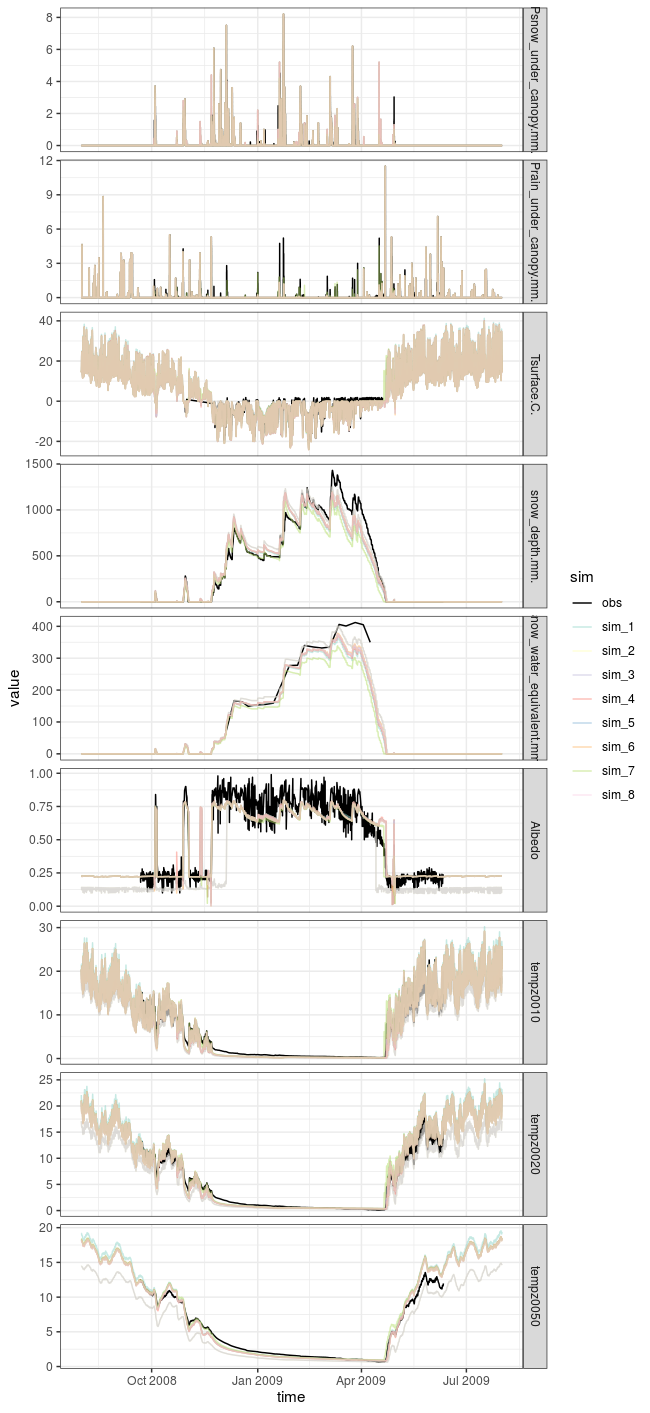
\includegraphics{coldelaporte_v6_files/figure-latex/Winter_2008_2009-1.png}

Goodness of fit:

\begin{longtable}[]{@{}llrrrrrrrrr@{}}
\toprule
sim & gof & Psnow\_under\_canopy.mm. & Prain\_under\_canopy.mm. &
Tsurface.C. & snow\_depth.mm. & snow\_water\_equivalent.mm. & Albedo &
tempz0010 & tempz0020 & tempz0050\tabularnewline
\midrule
\endhead
obs & MAE & 0.03 & 0.02 & 0.00 & 0.00 & 0.00 & 0.00 & 0.00 & 0.00 &
0.00\tabularnewline
obs & RMSE & 0.24 & 0.20 & 0.00 & 0.00 & 0.00 & 0.01 & 0.00 & 0.00 &
0.00\tabularnewline
obs & KGE & 0.74 & 0.92 & 1.00 & 1.00 & 1.00 & 1.00 & 1.00 & 1.00 &
1.00\tabularnewline
sim\_1 & MAE & 0.06 & 0.08 & 1.43 & 66.87 & 35.07 & 0.06 & 0.69 & 0.64 &
0.55\tabularnewline
sim\_1 & RMSE & 0.33 & 0.45 & 1.97 & 112.51 & 54.74 & 0.09 & 0.96 & 0.96
& 0.78\tabularnewline
sim\_1 & KGE & 0.47 & 0.59 & 0.85 & 0.88 & 0.73 & 0.87 & 0.89 & 0.86 &
0.85\tabularnewline
sim\_2 & MAE & 0.06 & 0.09 & 1.82 & 60.05 & 25.47 & 0.13 & 1.35 & 1.13 &
1.25\tabularnewline
sim\_2 & RMSE & 0.34 & 0.48 & 2.55 & 90.57 & 35.98 & 0.19 & 1.95 & 1.56
& 1.49\tabularnewline
sim\_2 & KGE & 0.47 & 0.51 & 0.82 & 0.96 & 0.85 & 0.72 & 0.66 & 0.71 &
0.70\tabularnewline
sim\_3 & MAE & 0.06 & 0.09 & 1.82 & 60.05 & 25.47 & 0.13 & 1.35 & 1.13 &
1.25\tabularnewline
sim\_3 & RMSE & 0.34 & 0.48 & 2.55 & 90.57 & 35.98 & 0.19 & 1.95 & 1.56
& 1.49\tabularnewline
sim\_3 & KGE & 0.47 & 0.51 & 0.82 & 0.96 & 0.85 & 0.72 & 0.66 & 0.71 &
0.70\tabularnewline
sim\_4 & MAE & 0.07 & 0.09 & 1.82 & 63.43 & 31.64 & 0.06 & 0.73 & 0.64 &
0.53\tabularnewline
sim\_4 & RMSE & 0.37 & 0.49 & 2.52 & 104.30 & 50.86 & 0.09 & 1.06 & 0.94
& 0.73\tabularnewline
sim\_4 & KGE & 0.39 & 0.52 & 0.81 & 0.90 & 0.75 & 0.87 & 0.90 & 0.88 &
0.87\tabularnewline
sim\_5 & MAE & 0.07 & 0.09 & 1.79 & 61.20 & 29.53 & 0.06 & 0.70 & 0.61 &
0.51\tabularnewline
sim\_5 & RMSE & 0.37 & 0.49 & 2.49 & 100.75 & 47.63 & 0.09 & 0.99 & 0.89
& 0.70\tabularnewline
sim\_5 & KGE & 0.39 & 0.52 & 0.81 & 0.91 & 0.77 & 0.86 & 0.90 & 0.89 &
0.88\tabularnewline
sim\_6 & MAE & 0.07 & 0.09 & 1.79 & 59.79 & 28.13 & 0.06 & 0.70 & 0.61 &
0.51\tabularnewline
sim\_6 & RMSE & 0.37 & 0.49 & 2.48 & 98.27 & 45.53 & 0.09 & 0.99 & 0.88
& 0.70\tabularnewline
sim\_6 & KGE & 0.39 & 0.52 & 0.81 & 0.91 & 0.78 & 0.86 & 0.90 & 0.89 &
0.88\tabularnewline
sim\_7 & MAE & 0.06 & 0.10 & 1.76 & 77.73 & 51.91 & 0.06 & 0.69 & 0.62 &
0.50\tabularnewline
sim\_7 & RMSE & 0.35 & 0.49 & 2.45 & 140.81 & 72.10 & 0.08 & 1.03 & 0.95
& 0.74\tabularnewline
sim\_7 & KGE & 0.48 & 0.55 & 0.83 & 0.78 & 0.64 & 0.86 & 0.90 & 0.87 &
0.86\tabularnewline
sim\_8 & MAE & 0.07 & 0.09 & 1.79 & 61.20 & 29.53 & 0.06 & 0.70 & 0.61 &
0.51\tabularnewline
sim\_8 & RMSE & 0.37 & 0.49 & 2.49 & 100.75 & 47.63 & 0.09 & 0.99 & 0.89
& 0.70\tabularnewline
sim\_8 & KGE & 0.39 & 0.52 & 0.81 & 0.91 & 0.77 & 0.86 & 0.90 & 0.89 &
0.88\tabularnewline
\bottomrule
\end{longtable}

\hypertarget{winter-20092010}{%
\subsubsection{Winter 2009/2010}\label{winter-20092010}}

Here is a comparison plot:

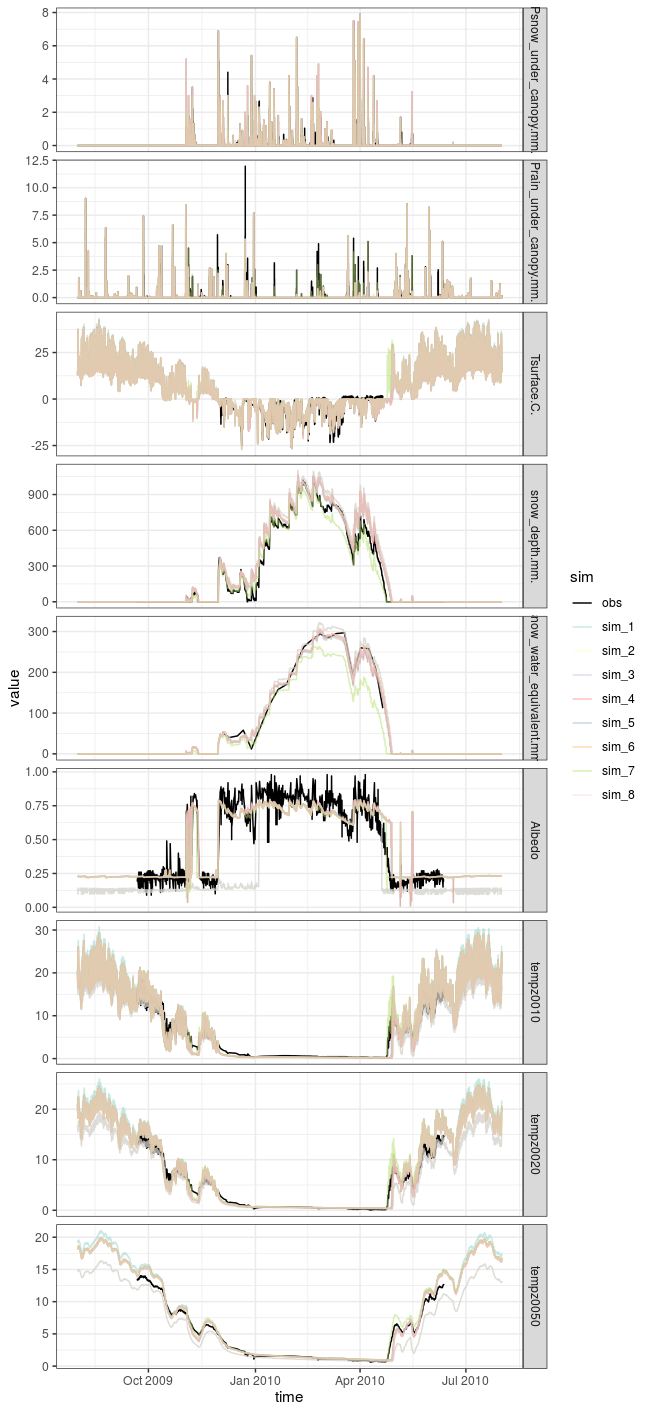
\includegraphics{coldelaporte_v6_files/figure-latex/Winter_2009_2010-1.png}

Goodness of fit:

\begin{longtable}[]{@{}llrrrrrrrrr@{}}
\toprule
sim & gof & Psnow\_under\_canopy.mm. & Prain\_under\_canopy.mm. &
Tsurface.C. & snow\_depth.mm. & snow\_water\_equivalent.mm. & Albedo &
tempz0010 & tempz0020 & tempz0050\tabularnewline
\midrule
\endhead
obs & MAE & 0.03 & 0.05 & 0.00 & 0.00 & 0.00 & 0.00 & 0.00 & 0.00 &
0.00\tabularnewline
obs & RMSE & 0.23 & 0.32 & 0.00 & 0.00 & 0.00 & 0.01 & 0.00 & 0.00 &
0.00\tabularnewline
obs & KGE & 0.78 & 0.83 & 1.00 & 1.00 & 1.00 & 1.00 & 1.00 & 1.00 &
1.00\tabularnewline
sim\_1 & MAE & 0.07 & 0.11 & 1.71 & 42.53 & 15.25 & 0.06 & 0.95 & 0.81 &
0.52\tabularnewline
sim\_1 & RMSE & 0.39 & 0.53 & 2.27 & 70.34 & 17.42 & 0.10 & 1.61 & 1.33
& 0.82\tabularnewline
sim\_1 & KGE & 0.34 & 0.48 & 0.84 & 0.86 & 0.92 & 0.89 & 0.79 & 0.80 &
0.86\tabularnewline
sim\_2 & MAE & 0.08 & 0.12 & 2.04 & 65.03 & 16.57 & 0.15 & 1.04 & 0.87 &
1.01\tabularnewline
sim\_2 & RMSE & 0.41 & 0.59 & 2.82 & 99.03 & 20.53 & 0.23 & 1.66 & 1.40
& 1.39\tabularnewline
sim\_2 & KGE & 0.31 & 0.37 & 0.80 & 0.75 & 0.93 & 0.64 & 0.74 & 0.78 &
0.75\tabularnewline
sim\_3 & MAE & 0.08 & 0.12 & 2.04 & 65.03 & 16.57 & 0.15 & 1.04 & 0.87 &
1.01\tabularnewline
sim\_3 & RMSE & 0.41 & 0.59 & 2.82 & 99.03 & 20.53 & 0.23 & 1.66 & 1.40
& 1.39\tabularnewline
sim\_3 & KGE & 0.31 & 0.37 & 0.80 & 0.75 & 0.93 & 0.64 & 0.74 & 0.78 &
0.75\tabularnewline
sim\_4 & MAE & 0.08 & 0.12 & 1.99 & 44.86 & 15.22 & 0.07 & 0.94 & 0.78 &
0.47\tabularnewline
sim\_4 & RMSE & 0.44 & 0.60 & 2.75 & 74.39 & 17.53 & 0.10 & 1.63 & 1.30
& 0.75\tabularnewline
sim\_4 & KGE & 0.23 & 0.37 & 0.83 & 0.84 & 0.93 & 0.89 & 0.80 & 0.82 &
0.89\tabularnewline
sim\_5 & MAE & 0.08 & 0.12 & 1.96 & 47.64 & 14.02 & 0.07 & 0.92 & 0.76 &
0.46\tabularnewline
sim\_5 & RMSE & 0.44 & 0.60 & 2.70 & 78.76 & 16.90 & 0.10 & 1.60 & 1.27
& 0.73\tabularnewline
sim\_5 & KGE & 0.23 & 0.37 & 0.83 & 0.83 & 0.94 & 0.88 & 0.81 & 0.83 &
0.90\tabularnewline
sim\_6 & MAE & 0.08 & 0.12 & 1.96 & 47.99 & 13.69 & 0.07 & 0.92 & 0.75 &
0.46\tabularnewline
sim\_6 & RMSE & 0.44 & 0.60 & 2.69 & 79.29 & 16.91 & 0.10 & 1.59 & 1.26
& 0.73\tabularnewline
sim\_6 & KGE & 0.23 & 0.37 & 0.84 & 0.82 & 0.95 & 0.88 & 0.81 & 0.83 &
0.90\tabularnewline
sim\_7 & MAE & 0.07 & 0.13 & 1.96 & 32.97 & 38.15 & 0.06 & 0.94 & 0.82 &
0.51\tabularnewline
sim\_7 & RMSE & 0.41 & 0.60 & 2.70 & 55.81 & 47.48 & 0.09 & 1.59 & 1.34
& 0.76\tabularnewline
sim\_7 & KGE & 0.38 & 0.41 & 0.82 & 0.90 & 0.73 & 0.88 & 0.77 & 0.78 &
0.85\tabularnewline
sim\_8 & MAE & 0.08 & 0.12 & 1.96 & 47.64 & 14.02 & 0.07 & 0.92 & 0.76 &
0.46\tabularnewline
sim\_8 & RMSE & 0.44 & 0.60 & 2.70 & 78.76 & 16.90 & 0.10 & 1.60 & 1.27
& 0.73\tabularnewline
sim\_8 & KGE & 0.23 & 0.37 & 0.83 & 0.83 & 0.94 & 0.88 & 0.81 & 0.83 &
0.90\tabularnewline
\bottomrule
\end{longtable}

\hypertarget{winter-20102011}{%
\subsubsection{Winter 2010/2011}\label{winter-20102011}}

Here is a comparison plot:

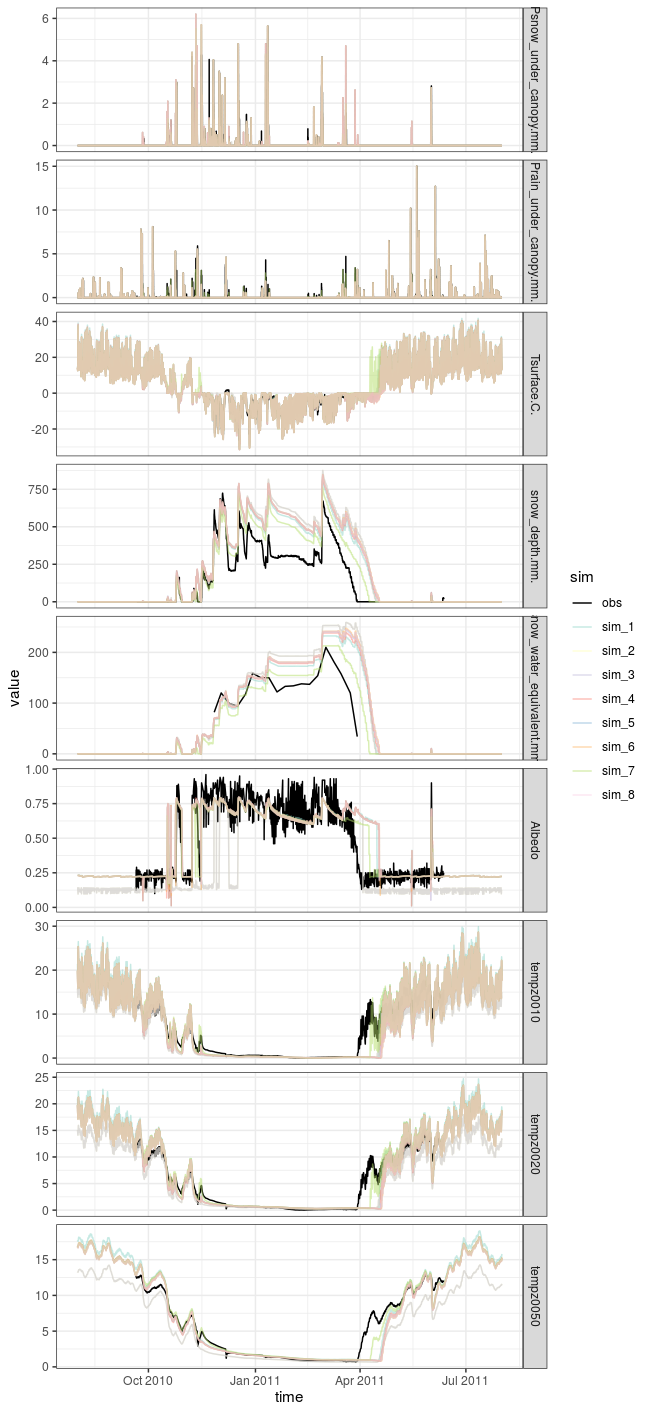
\includegraphics{coldelaporte_v6_files/figure-latex/Winter_2010_2011-1.png}

Goodness of fit:

\begin{longtable}[]{@{}llrrrrrrrrr@{}}
\toprule
sim & gof & Psnow\_under\_canopy.mm. & Prain\_under\_canopy.mm. &
Tsurface.C. & snow\_depth.mm. & snow\_water\_equivalent.mm. & Albedo &
tempz0010 & tempz0020 & tempz0050\tabularnewline
\midrule
\endhead
obs & MAE & 0.02 & 0.04 & 0.00 & 0.00 & 0.00 & 0.00 & 0.00 & 0.00 &
0.00\tabularnewline
obs & RMSE & 0.18 & 0.33 & 0.00 & 0.00 & 0.00 & 0.01 & 0.00 & 0.00 &
0.00\tabularnewline
obs & KGE & 0.78 & 0.83 & 1.00 & 1.00 & 1.00 & 1.00 & 1.00 & 1.00 &
1.00\tabularnewline
sim\_1 & MAE & 0.05 & 0.11 & 2.10 & 108.04 & 39.30 & 0.08 & 1.33 & 1.12
& 0.82\tabularnewline
sim\_1 & RMSE & 0.30 & 0.57 & 2.71 & 156.99 & 55.54 & 0.15 & 2.45 & 2.02
& 1.53\tabularnewline
sim\_1 & KGE & 0.29 & 0.49 & 0.72 & 0.30 & 0.35 & 0.80 & 0.80 & 0.86 &
0.90\tabularnewline
sim\_2 & MAE & 0.05 & 0.13 & 2.53 & 132.29 & 53.02 & 0.15 & 1.58 & 1.42
& 1.58\tabularnewline
sim\_2 & RMSE & 0.26 & 0.61 & 3.30 & 192.65 & 72.80 & 0.22 & 2.59 & 2.30
& 2.22\tabularnewline
sim\_2 & KGE & 0.43 & 0.40 & 0.72 & 0.13 & 0.14 & 0.64 & 0.64 & 0.67 &
0.63\tabularnewline
sim\_3 & MAE & 0.05 & 0.13 & 2.53 & 132.29 & 53.02 & 0.15 & 1.58 & 1.42
& 1.58\tabularnewline
sim\_3 & RMSE & 0.26 & 0.61 & 3.30 & 192.65 & 72.80 & 0.22 & 2.59 & 2.30
& 2.22\tabularnewline
sim\_3 & KGE & 0.43 & 0.40 & 0.72 & 0.13 & 0.14 & 0.64 & 0.64 & 0.67 &
0.63\tabularnewline
sim\_4 & MAE & 0.06 & 0.13 & 2.45 & 118.39 & 42.56 & 0.09 & 1.38 & 1.13
& 0.83\tabularnewline
sim\_4 & RMSE & 0.32 & 0.62 & 3.17 & 170.92 & 60.16 & 0.15 & 2.52 & 2.06
& 1.59\tabularnewline
sim\_4 & KGE & 0.23 & 0.40 & 0.70 & 0.22 & 0.30 & 0.79 & 0.80 & 0.86 &
0.88\tabularnewline
sim\_5 & MAE & 0.06 & 0.13 & 2.44 & 120.66 & 44.47 & 0.09 & 1.38 & 1.12
& 0.83\tabularnewline
sim\_5 & RMSE & 0.32 & 0.62 & 3.15 & 174.23 & 63.06 & 0.15 & 2.52 & 2.07
& 1.61\tabularnewline
sim\_5 & KGE & 0.23 & 0.40 & 0.69 & 0.21 & 0.26 & 0.79 & 0.80 & 0.86 &
0.88\tabularnewline
sim\_6 & MAE & 0.06 & 0.13 & 2.44 & 121.96 & 45.04 & 0.09 & 1.38 & 1.12
& 0.83\tabularnewline
sim\_6 & RMSE & 0.32 & 0.62 & 3.15 & 176.18 & 64.04 & 0.15 & 2.53 & 2.07
& 1.62\tabularnewline
sim\_6 & KGE & 0.23 & 0.40 & 0.68 & 0.20 & 0.24 & 0.78 & 0.80 & 0.86 &
0.88\tabularnewline
sim\_7 & MAE & 0.05 & 0.13 & 2.42 & 75.23 & 27.78 & 0.06 & 1.11 & 0.90 &
0.64\tabularnewline
sim\_7 & RMSE & 0.28 & 0.62 & 3.13 & 112.34 & 35.66 & 0.11 & 2.01 & 1.58
& 1.15\tabularnewline
sim\_7 & KGE & 0.48 & 0.43 & 0.70 & 0.55 & 0.61 & 0.86 & 0.85 & 0.89 &
0.94\tabularnewline
sim\_8 & MAE & 0.06 & 0.13 & 2.44 & 120.66 & 44.47 & 0.09 & 1.38 & 1.12
& 0.83\tabularnewline
sim\_8 & RMSE & 0.32 & 0.62 & 3.15 & 174.23 & 63.06 & 0.15 & 2.52 & 2.07
& 1.61\tabularnewline
sim\_8 & KGE & 0.23 & 0.40 & 0.69 & 0.21 & 0.26 & 0.79 & 0.80 & 0.86 &
0.88\tabularnewline
\bottomrule
\end{longtable}

\hypertarget{references}{%
\subsubsection*{References}\label{references}}
\addcontentsline{toc}{subsubsection}{References}

\hypertarget{refs}{}
\begin{cslreferences}
\leavevmode\hypertarget{ref-Endrizzi2014}{}%
Endrizzi, S., S. Gruber, M. Dall'Amico, and R. Rigon. 2014. ``GEOtop
2.0: Simulating the Combined Energy and Water Balance at and Below the
Land Surface Accounting for Soil Freezing, Snow Cover and Terrain
Effects.'' \emph{Geoscientific Model Development} 7 (6): 2831--57.
\url{https://doi.org/10.5194/gmd-7-2831-2014}.

\leavevmode\hypertarget{ref-Morin2012}{}%
Morin, S., Y. Lejeune, B. Lesaffre, J.-M. Panel, D. Poncet, P. David,
and M. Sudul. 2012. ``An 18-Yr Long (1993â€``2011) Snow and
Meteorological Dataset from a Mid-Altitude Mountain Site (Col de Porte,
France, 1325 M Alt.) for Driving and Evaluating Snowpack Models.''
\emph{Earth System Science Data} 4 (1): 13--21.
\url{https://doi.org/10.5194/essd-4-13-2012}.
\end{cslreferences}

\end{document}
